\section{FESDModelv1 Results}
\label{sec:FESDModelv1_results}

After training all four models using FESDModelv1, the results are evaluated. Table \ref{tab:res_v1} shows the results of the testing after 100 epochs of training. The results seem promising with an accuracy in the range of 80 to 90 percent. Additionally, the Cohen's Kappa coefficient shows results in a good range.

\begin{table}
  \caption[Test Results of FESDModelv1]{The test results of FESDModelv1 after 100 epochs of training.}
  \label{tab:res_v1}
  \centering
  \begin{tabular}{p{0.15\linewidth}p{0.15\linewidth}p{0.15\linewidth}p{0.15\linewidth}p{0.15\linewidth}}
    \hline
    {} &  Percentage of positive guesses &  Accuracy &  F1-Score &  Cohen's Kappa Coefficient \\
    Problem Set   &                                 &           &           &                            \\
    \hline
    Full Body  &                          71.667 &     0.842 &     0.642 &                      0.528 \\
    Half Body  &                          64.375 &     0.840 &     0.525 &                      0.622 \\
    Body Parts &                          93.681 &     0.917 &     0.864 &                      0.677 \\
    Joints     &                          69.990 &     0.893 &     0.638 &                      0.773 \\
    \hline
  \end{tabular}
\end{table}

To understand these results the cofusion matrix and ROC curve were calculated. The confusion matrices can be seen in figure \ref{fig:conf_v1} and ROC curves can be seen in figure \ref{fig:roc_v1}. The confusion matrix seems to reflect the results of table \ref{tab:res_v1}. However, the ROC curve shows that the results are as good as they are due to overconfidence and possibly overfitting of the data.

\begin{figure}[ht]
  \centering
  \begin{subfigure}[b]{0.47\linewidth}
      \centering
      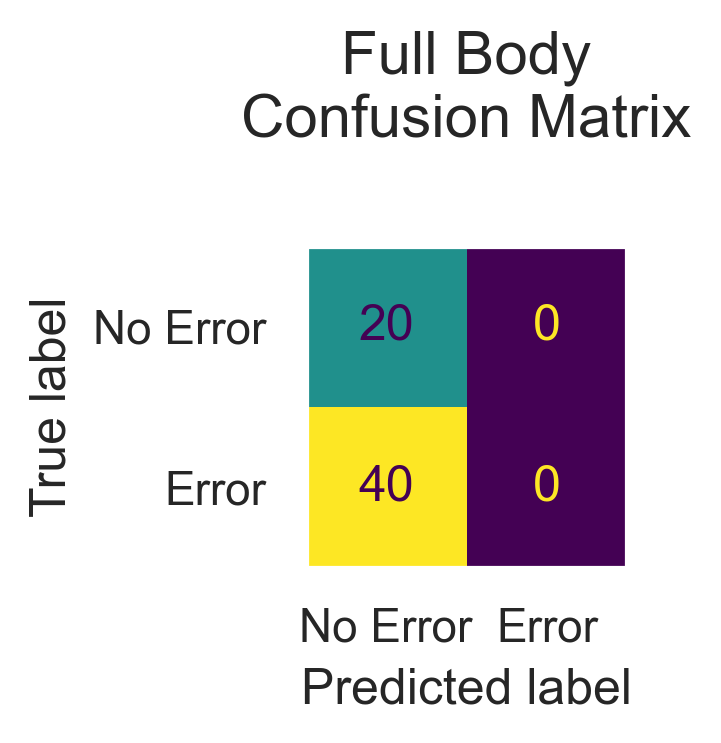
\includegraphics[width=\textwidth]{figures/Results/v1/confusion/full_together.png}
      \caption[]{Full Body Problem Set}
      \label{fig:fb_conf_v1}
  \end{subfigure}
  \hfill
  \begin{subfigure}[b]{0.47\linewidth}
      \centering
      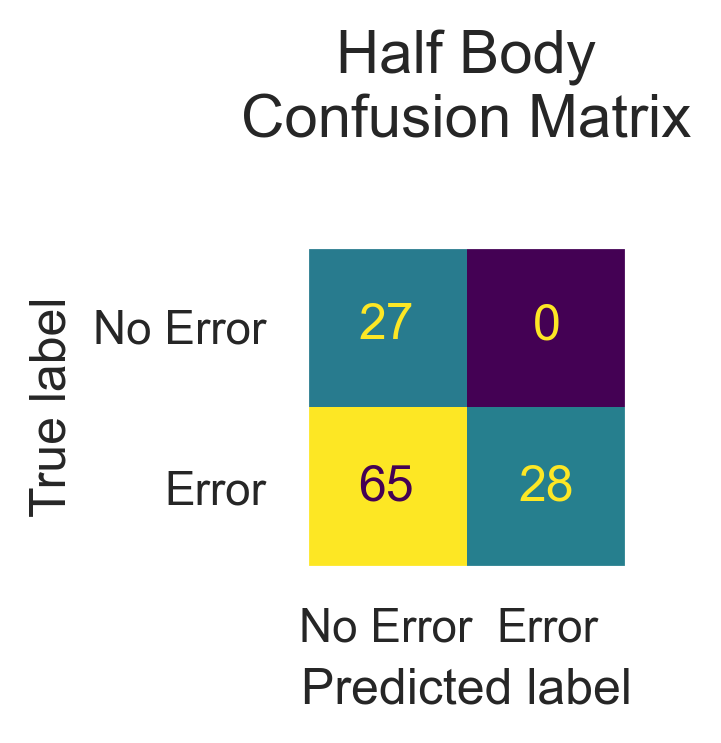
\includegraphics[width=\textwidth]{figures/Results/v1/confusion/half_together.png}
      \caption[]{Half Body Problem Set}
      \label{fig:hb_conf_v1}
  \end{subfigure}
  \hfill
  \begin{subfigure}[b]{0.47\linewidth}
      \centering
      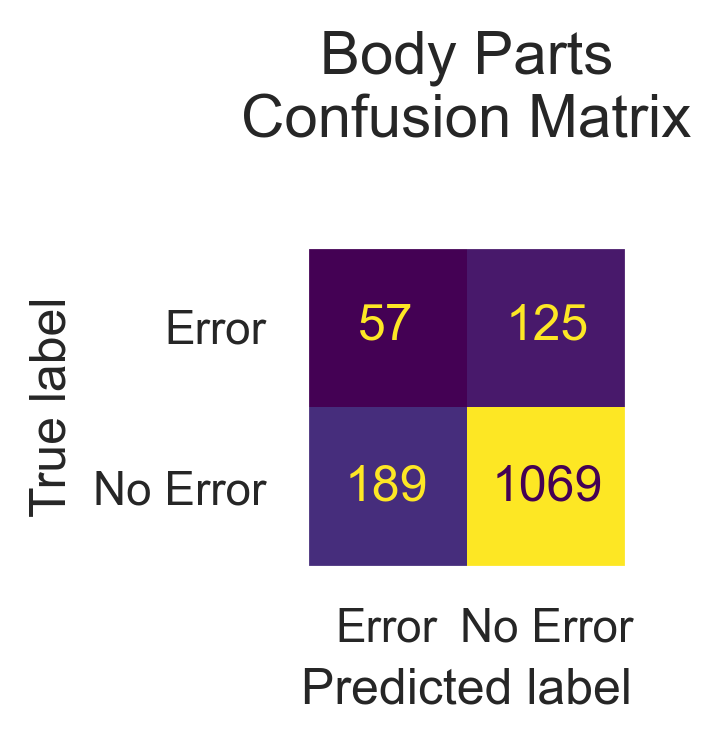
\includegraphics[width=\textwidth]{figures/Results/v1/confusion/body_parts_together.png}
      \caption[]{Body Part Problem Set}
      \label{fig:bp_conf_v1}
  \end{subfigure}
  \hfill
  \begin{subfigure}[b]{0.47\linewidth}
      \centering
      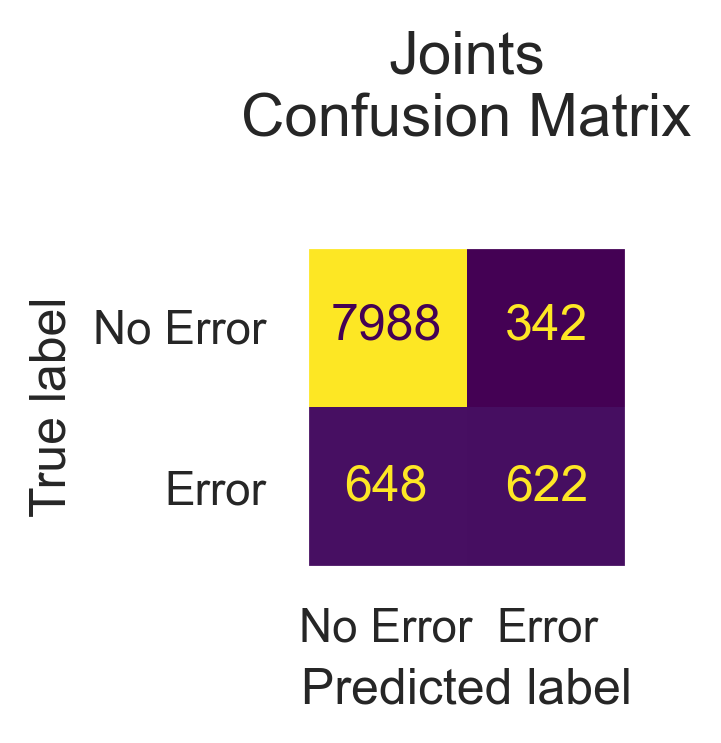
\includegraphics[width=\textwidth]{figures/Results/v1/confusion/joints_together.png}
      \caption[]{Joint Problem Set}
      \label{fig:jt_conf_v1}
  \end{subfigure}
  \caption[Confusion Matrices of FESDModelv1]{The confusion Matrices of FESDModelv1.}
  \label{fig:conf_v1}
\end{figure}

\begin{figure}
  \centering
  \begin{subfigure}[b]{0.47\linewidth}
      \centering
      \includegraphics[width=\textwidth]{figures/Results/v1/fb/roc.png}
      \caption[]{Full Body Problem Set}
      \label{fig:fb_roc_v1}
  \end{subfigure}
  \hfill
  \begin{subfigure}[b]{0.47\linewidth}
      \centering
      \includegraphics[width=\textwidth]{figures/Results/v1/hb/roc.png}
      \caption[]{Half Body Problem Set}
      \label{fig:hb_roc_v1}
  \end{subfigure}
  \hfill
  \begin{subfigure}[b]{0.47\linewidth}
      \centering
      \includegraphics[width=\textwidth]{figures/Results/v1/bp/roc.png}
      \caption[]{Body Part Problem Set}
      \label{fig:bp_roc_v1}
  \end{subfigure}
  \hfill
  \begin{subfigure}[b]{0.47\linewidth}
      \centering
      \includegraphics[width=\textwidth]{figures/Results/v1/jt/roc.png}
      \caption[]{Joint Problem Set}
      \label{fig:jt_roc_v1}
  \end{subfigure}
  \caption[ROC Curves of FESDModelv1]{The ROC curves of FESDModelv1.}
  \label{fig:roc_v1}
\end{figure}

The results for the table and the confusion matrices were summarised over all areas in a problem set, therefore, these seemingly positive values occur. If the areas are considered individually it can be seen that the model is overfitting for each of the areas and mainly predicting a single value. This produces good accuracy since the dataset is unbalanced.